% C++ and Java Program to Calculate Average of elements in an Integer Arrays. Take input values. Also display number of elements which are greater than average value.

\documentclass[11pt]{article}

% Preamble

\usepackage[margin=1in]{geometry}
\usepackage{amsfonts, amsmath, amssymb}
\usepackage{fancyhdr, float, graphicx}
\usepackage[utf8]{inputenc} % Required for inputting international characters
\usepackage[T1]{fontenc} % Output font encoding for international characters
\usepackage{fouriernc} % Use the New Century Schoolbook font
\usepackage[nottoc, notlot, notlof]{tocbibind}
\usepackage{listings}
\usepackage{xcolor}

\definecolor{codegreen}{rgb}{0,0.6,0}
\definecolor{codegray}{rgb}{0.5,0.5,0.5}
\definecolor{codepurple}{rgb}{0.58,0,0.82}
\definecolor{backcolour}{rgb}{0.95,0.95,0.92}

\lstdefinestyle{mystyle}{
    backgroundcolor=\color{backcolour},   
    commentstyle=\color{codegreen},
    keywordstyle=\color{magenta},
    numberstyle=\tiny\color{codegray},
    stringstyle=\color{codepurple},
    basicstyle=\ttfamily\footnotesize,
    breakatwhitespace=false,         
    breaklines=true,                 
    captionpos=b,                    
    keepspaces=true,                 
    numbers=left,                    
    numbersep=5pt,                  
    showspaces=false,                
    showstringspaces=false,
    showtabs=false,                  
    tabsize=2
}

\lstset{style=mystyle}

% Header and Footer
\pagestyle{fancy}
\fancyhead{}
\fancyfoot{}
\fancyhead[L]{\textit{\Large{OOPJC Case Study Report}}}
%\fancyhead[R]{\textit{something}}
\fancyfoot[C]{\thepage}
\renewcommand{\footrulewidth}{1pt}



% Other Doc Editing
% \parindent 0ex
%\renewcommand{\baselinestretch}{1.5}

\begin{document}

\begin{titlepage}
	\centering

	%---------------------------NAMES-------------------------------

	\huge\textsc{
		MIT World Peace University
	}\\

	\vspace{0.75\baselineskip} % space after Uni Name

	\LARGE{
		Object Oriented Programming with Java and C++\\
		Second Year B. Tech, Semester 1
	}

	\vfill % space after Sub Name

	%--------------------------TITLE-------------------------------

	\rule{\textwidth}{1.6pt}\vspace*{-\baselineskip}\vspace*{2pt}
	\rule{\textwidth}{0.6pt}
	\vspace{0.75\baselineskip} % Whitespace above the title



	\huge{\textsc{
			Case Study - Elements of an Array
		}} \\



	\vspace{0.5\baselineskip} % Whitespace below the title
	\rule{\textwidth}{0.6pt}\vspace*{-\baselineskip}\vspace*{2.8pt}
	\rule{\textwidth}{1.6pt}

	\vspace{1\baselineskip} % Whitespace after the title block

	%--------------------------SUBTITLE --------------------------	

	\LARGE\textsc{
		Project Report
	} % Subtitle or further description
	\vfill

	%--------------------------AUTHOR-------------------------------

	Prepared By
	\vspace{0.5\baselineskip} % Whitespace before the editors

	\Large{
		Krishnaraj Thadesar \\
		Cyber Security and Forensics\\
		Batch A1, PA 20
	}


	\vspace{0.5\baselineskip} % Whitespace below the editor list
	\today

\end{titlepage}


\tableofcontents
\thispagestyle{empty}
\clearpage


\setcounter{page}{1}
\section{Aim}
To perform a Case study on the given problem statement, and implement the problem in C++ and Java

\section{Problem Statement}
Write a C++ and Java Program to Calculate Average of elements in an Integer Arrays.Take input values.Also display number of elements which are greater than average value.


\section{Platform}
\textbf{Operating System}: Arch Linux x86-64 \\
\textbf{IDEs or Text Editors Used}: Visual Studio Code\\
\textbf{Compilers} : g++ and gcc on linux for C++, and javac, with JDK 18.0.2 for Java\\

\section{Flowchart}
\begin{figure}[H]
	\centering
	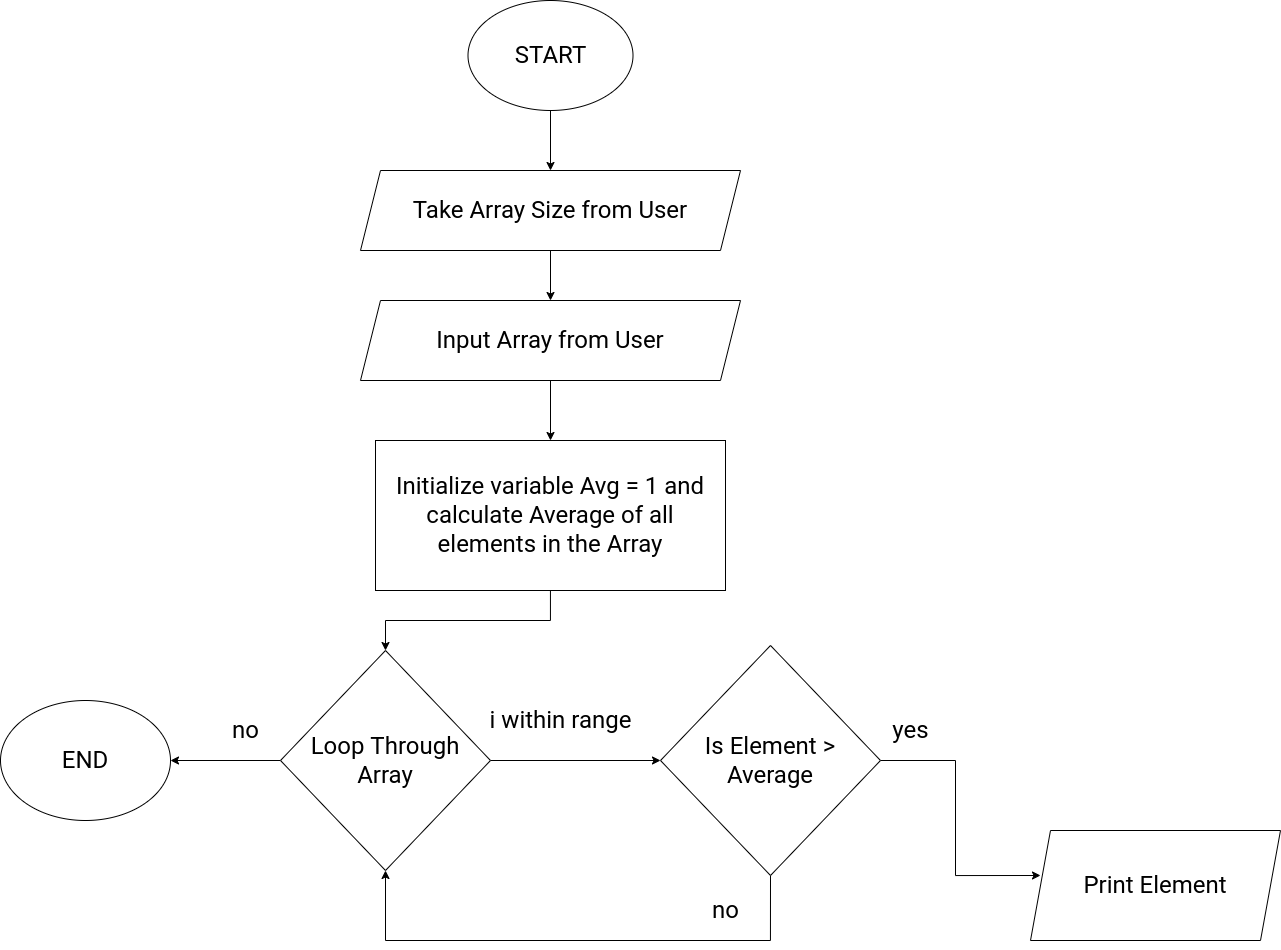
\includegraphics[scale=0.35]{flowchart.png}
	\caption{Flowchart for Algorithm}
\end{figure}

\section{Algorithm}
\begin{verbatim}
	STEP 1: Start
	STEP 2: Input Length of Array from user
	STEP 3: Input the Array from the user
	STEP 4: Initialize a variable avg to 1, and find average of Array
	STEP 5: Loop through the array, if element is greater than average then print it. 
	STEP 6: Exit. 
\end{verbatim}

\section{Code}
\subsection{C++ Implementation of Problem}
% \begin{figure}[H]
% 	\centering
% 	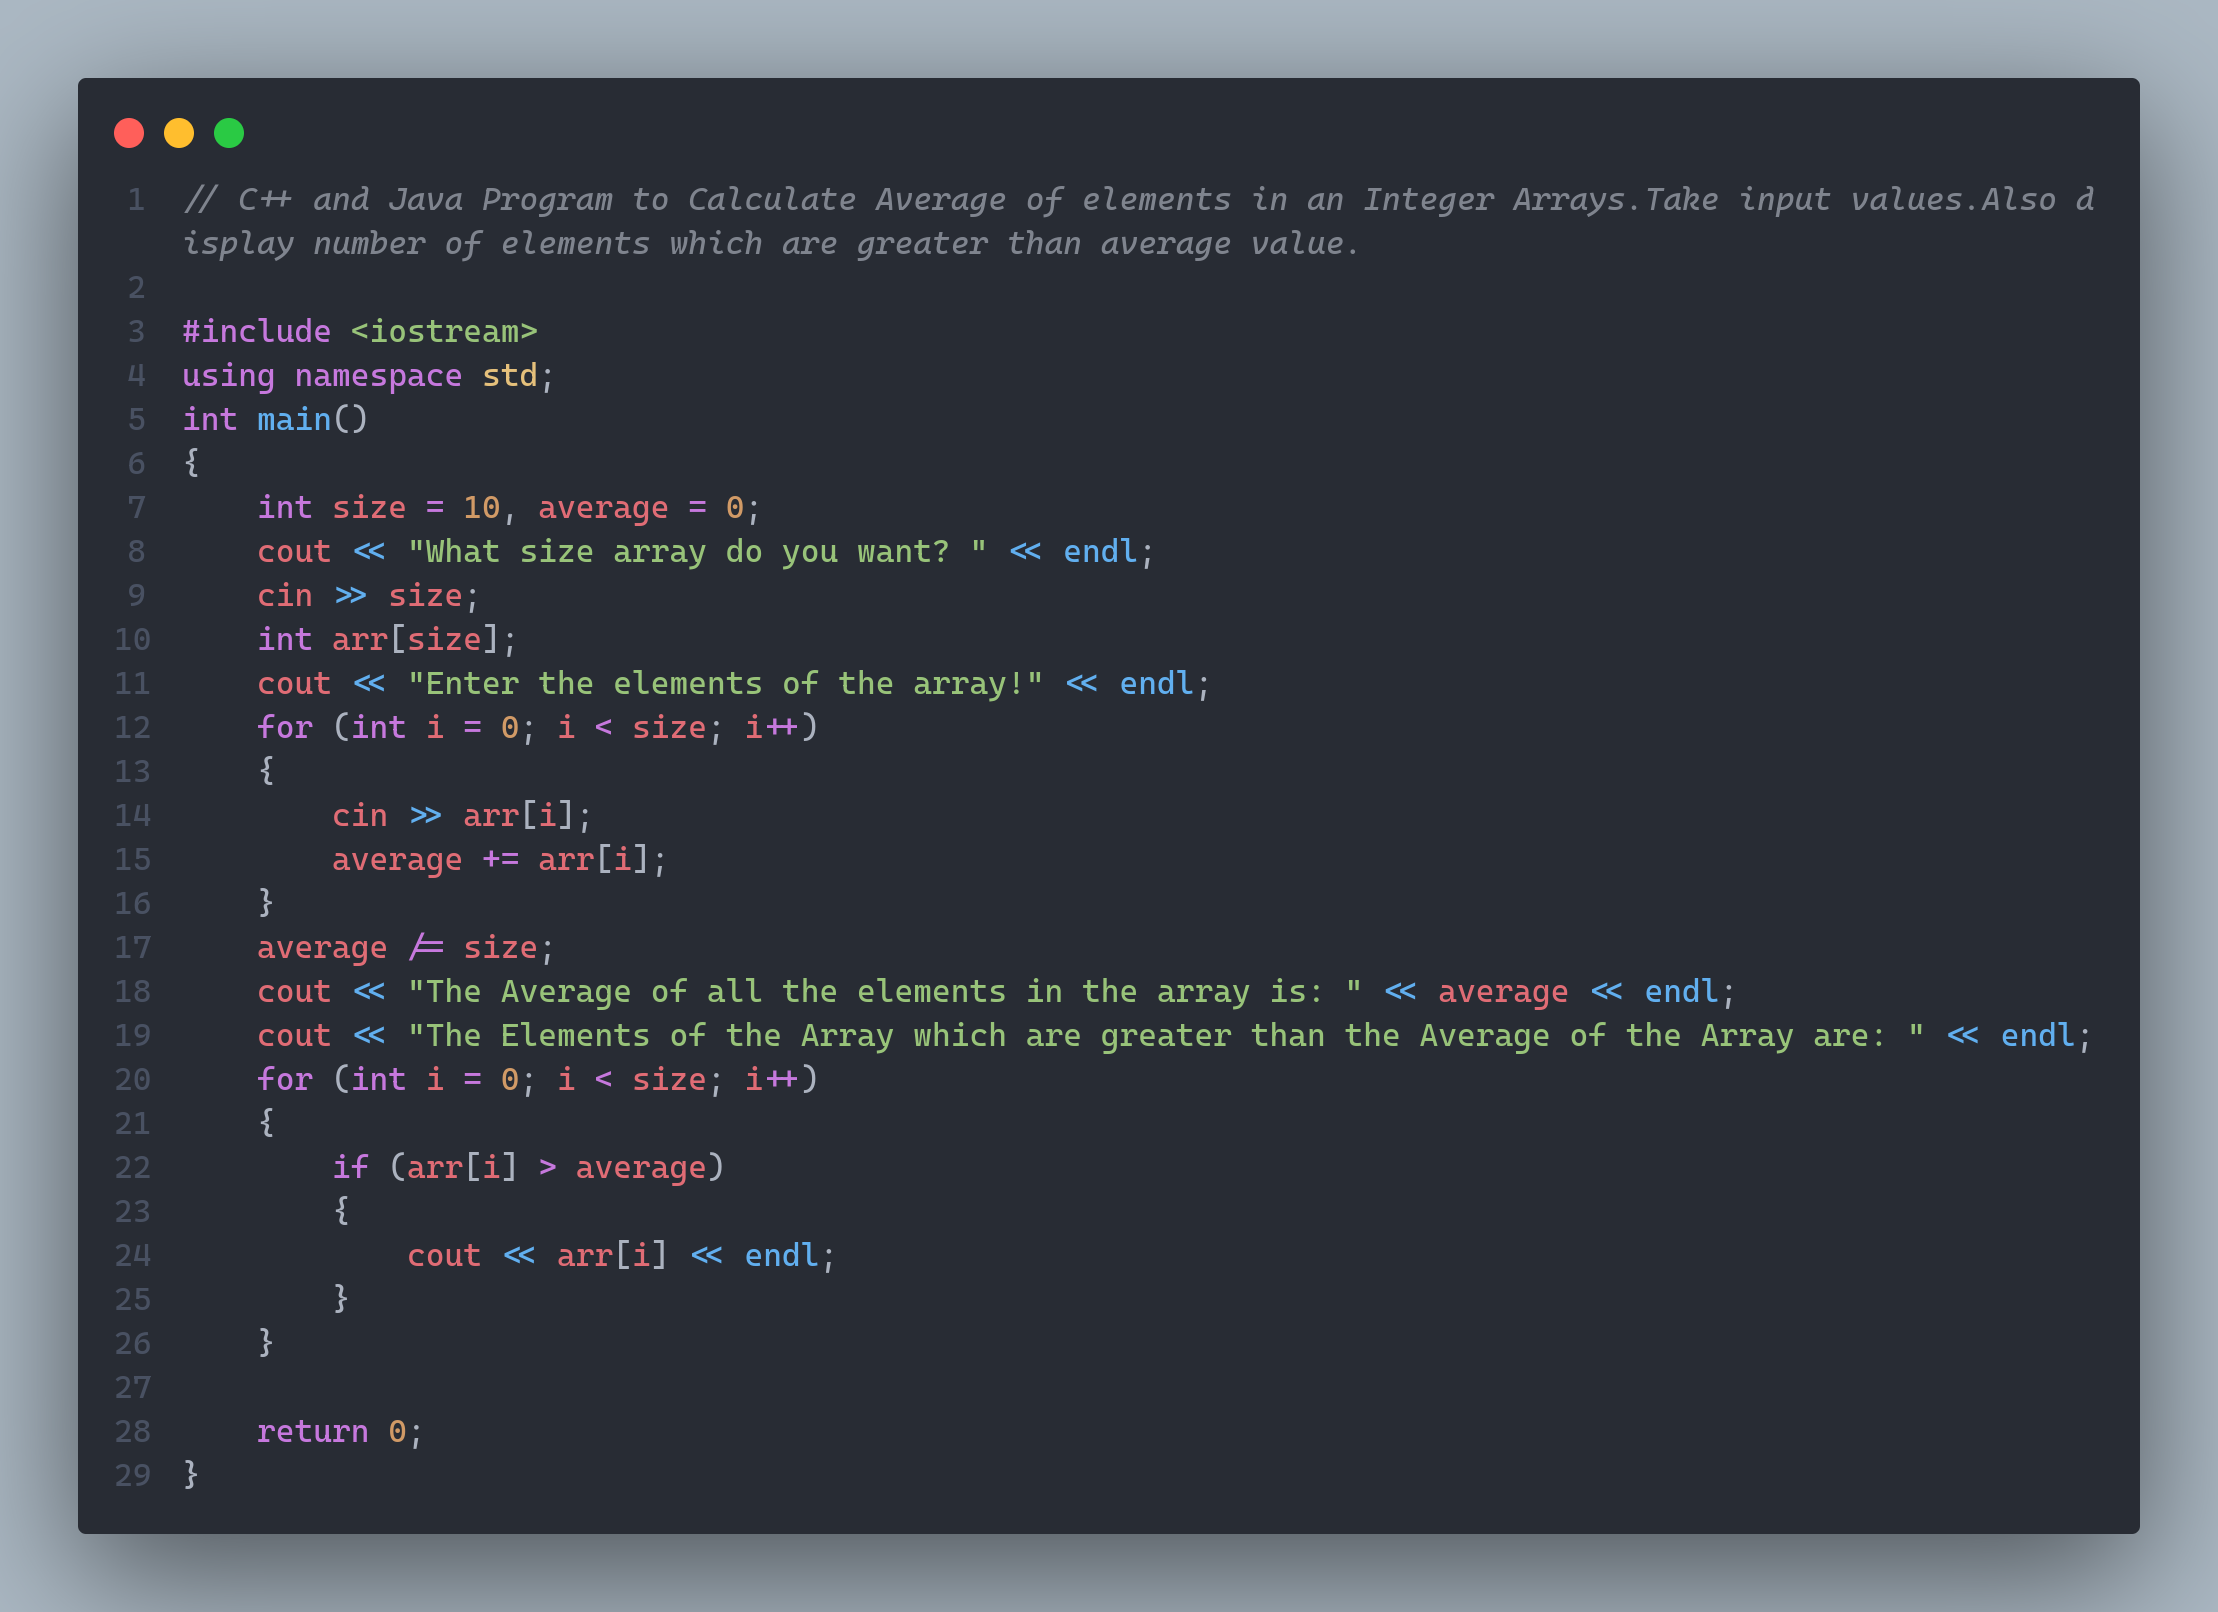
\includegraphics[scale=0.22]{codec.png}
% 	\caption{}
% \end{figure}
\lstinputlisting[language=c++, caption=Main.Cpp]{./case_study.cpp}

\subsection{Java Implementation of Problem}
% \begin{figure}[H]
% 	\centering
% 	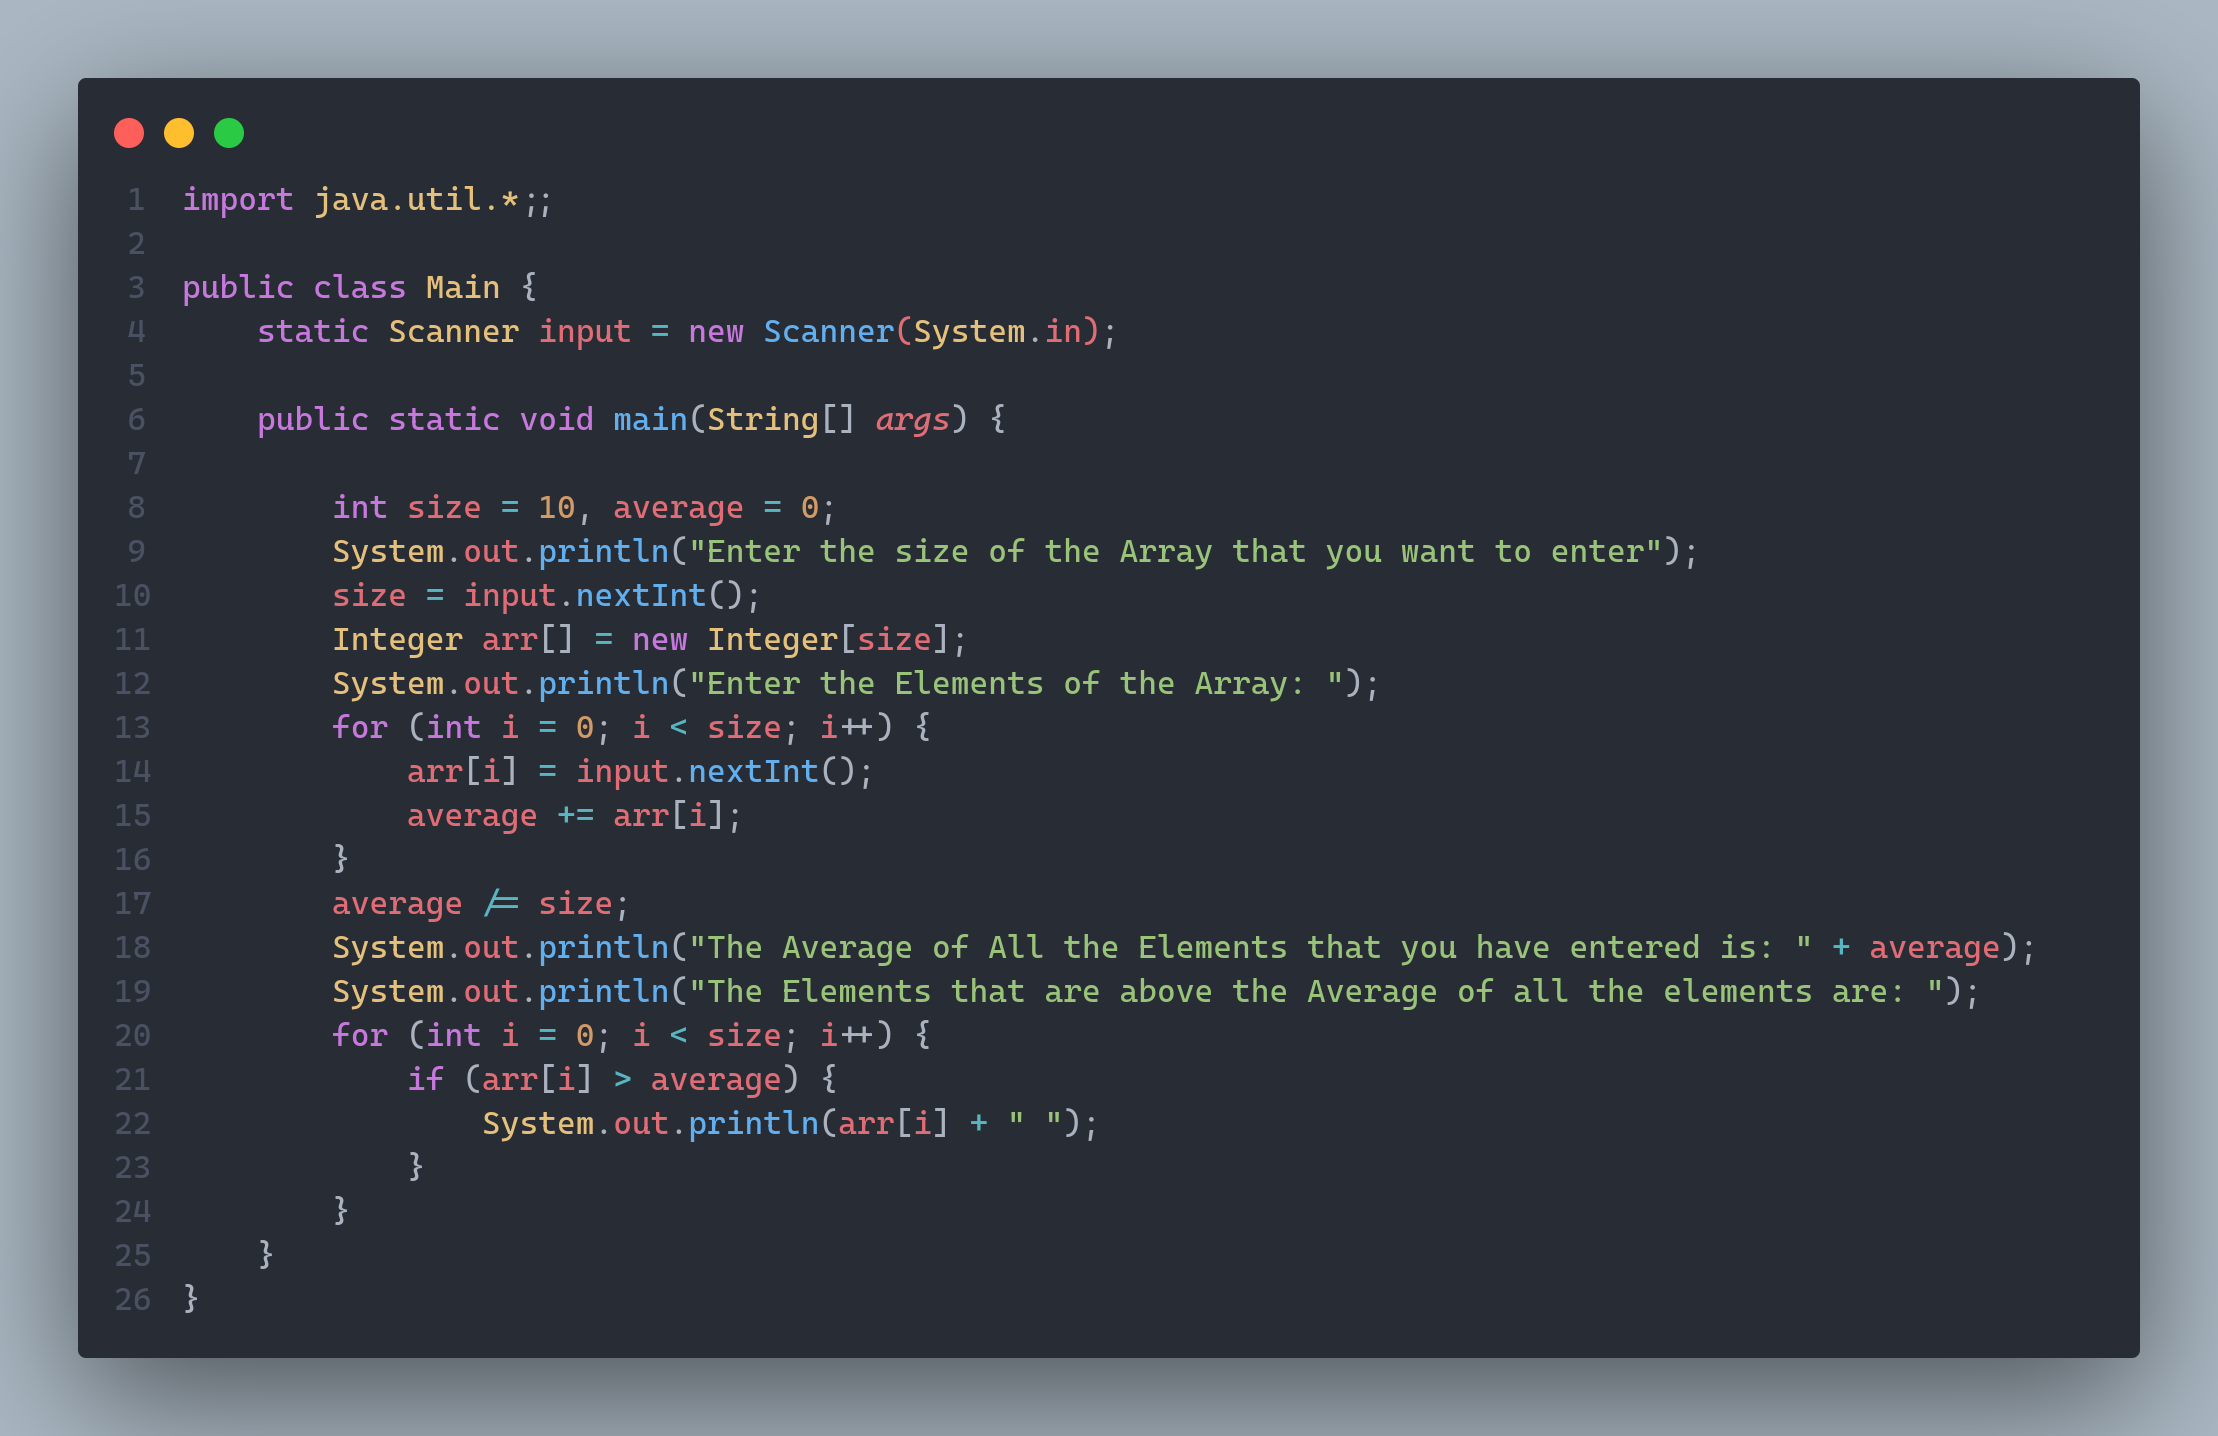
\includegraphics[scale=0.22]{code.png}
% 	\caption{}
% \end{figure}

\lstinputlisting[language=Java, caption=Main.java]{./Main.java}

\subsection{Input}1. What are the challenges for multithreading implementation using Java
Programming?
2. What is the difference between the start and run method in Java Thread?
3. Which one is better to implement thread in Java? extending Thread class or
implementing Runnable?
4. What is the difference between wait and sleep in Java? Explain with
example.
5. What is the difference between the submit() and execute() method of
Executor and ExecutorService in Java? Explain with example.
\begin{enumerate}
	\item Length of the Array
	\item The Elements of the Array
\end{enumerate}

\subsection{Output}

\subsection{C++ Output}
% \begin{figure}[H]
% 	\centering
% 	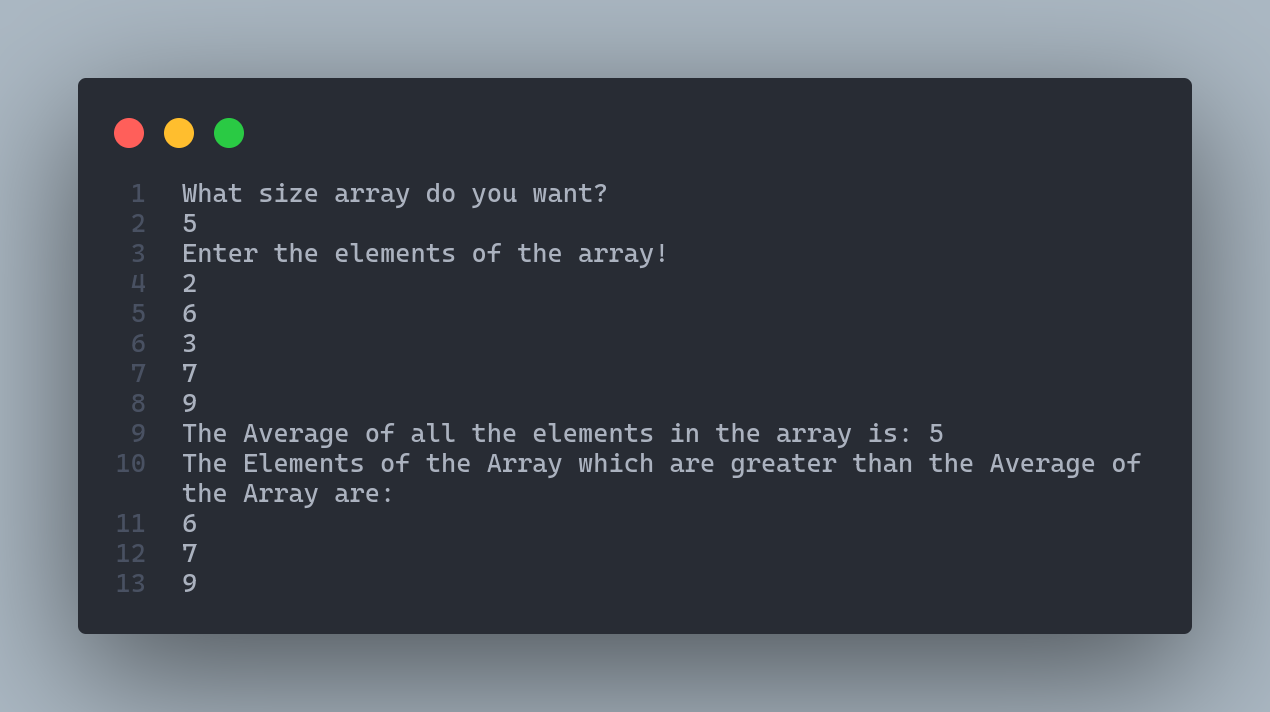
\includegraphics[scale=0.30]{output.png}
% 	\caption{}
% \end{figure}
\lstinputlisting[caption=Output for C++]{./case_study_output_cpp.txt}


\subsection{Java Output}
% \begin{figure}[H]
% 	\centering
% 	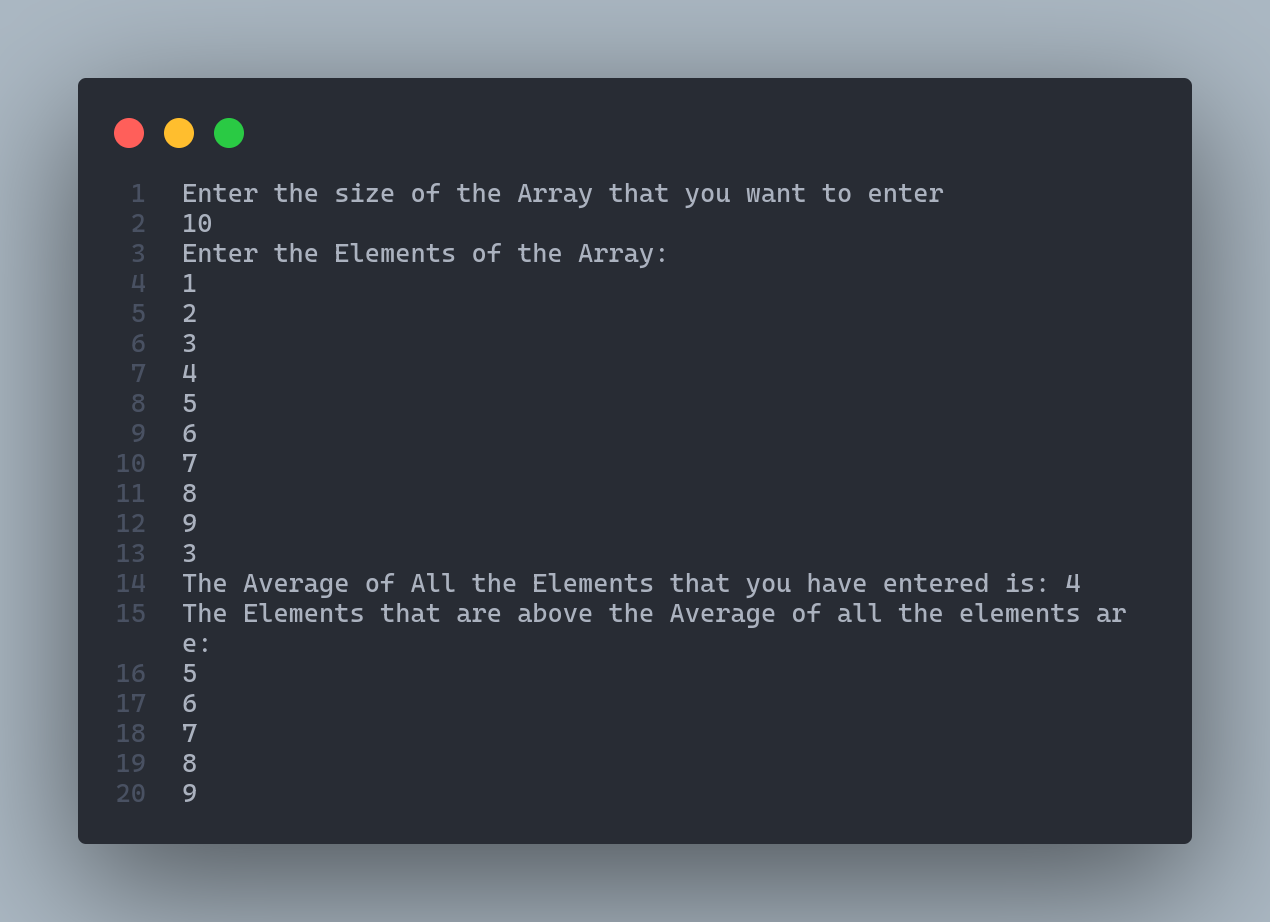
\includegraphics[scale=0.30]{outputj.png}
% 	\caption{}
% \end{figure}


\lstinputlisting[caption=Output for Java]{./case_study_output_java.txt}

\end{document}